\section{双层问题}
\label{sec:bilevel-problem}

外层目标依赖内层的最优解时，它到底是一个什么样的函数？先把两层的角色写下来。

外层变量记为$\bm{x}\in\bm{C}\subseteq\mathbb{R}^n$，内层变量记为$\bm{y}\in\mathbb{R}^d$。外层选定$\bm{x}$之后，内层在可行集$\bm{Y}(\bm{x})\subseteq\mathbb{R}^d$上最小化自己的目标$g$；外层再用另一个目标$F$评价内层的结果。

\begin{definition}[内层解集]
\label{def:bilevel-inner-solutions}
给定$\bm{x}\in\bm{C}$，称
\begin{equation}
 \bm{S}(\bm{x})=\argmin_{\bm{y}\in\bm{Y}(\bm{x})}g(\bm{x},\bm{y})
 \label{eq:bilevel-solution-set}
\end{equation}
为\term{内层解集}（lower-level solution set），其中的点称为内解。外层目标$F(\bm{x},\bm{y})$只对内解作评价，由此形成的嵌套问题称为\term{双层优化}（bilevel optimization）问题。
\end{definition}

图~\ref{fig:bilevel-structure}是这个结构的全貌。$\bm{x}$有两条路影响外层：一条直接进入$F$，另一条先改变内层问题，再通过选出的内解起作用。外层只能修改$\bm{x}$，不能直接修改$\bm{y}$。中间的“选解规则”一格是定义里没有出现、却必不可少的一步，第~\ref{sec:bilevel-selection}小节会讲它。

\begin{BookInlineFigure}
 \centering
 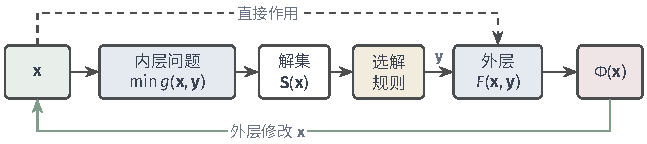
\includegraphics[width=109.6mm]{figures/05-optimization/07-multiple-criteria-and-nested-optimization/tikz/bilevel-structure/figure.pdf}
 \caption{双层问题的结构。外层变量$\bm{x}$决定内层问题，内层解集经选解规则给出$\bm{y}$，外层目标$F$再读取$\bm{y}$得到$\Phi(\bm{x})$。虚线是$\bm{x}$对$F$的直接作用，绿线表示外层根据$\Phi$修改$\bm{x}$。}
 \label{fig:bilevel-structure}
\end{BookInlineFigure}

\paragraph{内层无解时外层没有输入}
解集可能是空集。取外层变量$x\in\mathbb{R}$，内层变量$y\in\mathbb{R}$，内层目标是
\[
 g(x,y)=\frac{x}{2}y^2-y.
\]

$x>0$时这是开口向上的抛物线，唯一的内解是$y=1/x$。$x=0$时$g=-y$，$x<0$时$g$是开口向下的抛物线，两种情况下$y\to+\infty$都使$g\to-\infty$，内层没有最小点。

这时一个内层算法仍然可以运行并输出数字。比如梯度下降的更新是$y\leftarrow y+\alpha(1-xy)$，在$x<0$时迭代会不断增大。把这种数字交给外层，得到的外层值不评价任何内解。因此外层只在下面的集合上比较：
\begin{equation}
 \operatorname{dom}\bm{S}=\{\bm{x}\in\bm{C}:\bm{S}(\bm{x})\neq\varnothing\}.
 \label{eq:bilevel-dom}
\end{equation}
集合之外的$\bm{x}$一律视为外层不可行，外层值规定为$+\infty$。

\paragraph{与极小极大的区别}
第~\ref{chap:minimax-optimization}章的问题$\min_{\bm{x}}\max_{\bm{y}}f(\bm{x},\bm{y})$也是嵌套的，形式上取$g=-f$、$F=f$就是双层问题。可是那里两层围绕同一个代价相反地优化，内层的最优性恰好让外层目标对$\bm{y}$的偏导为零。双层问题的两个目标一般无关，内层最优并不让$F$在$\bm{y}$方向驻定，内解移动一点，外层值就跟着变化。表~\ref{tab:bilevel-vs-minimax}对比两者，第~\ref{sec:bilevel-hypergradient}小节会用公式说明最后一行。

\begin{BookInlineTable}
 \centering
 \begin{tabular}{lll}
  \toprule
  & 极小极大 & 双层优化\\
  \midrule
  内外目标 & 同一个$f$，方向相反 & $g$与$F$一般无关\\
  内解处$\nabla_{\bm{y}}F$ & 为零 & 一般不为零\\
  外层导数 & 无需内解的响应项 & 必须计入内解的响应\\
  \bottomrule
 \end{tabular}
 \caption{极小极大与双层优化的对比。第二、三行假定内解唯一、位于内层可行集内部且相关函数可微。}
 \label{tab:bilevel-vs-minimax}
\end{BookInlineTable}

\subsection{唯一内解}
\label{sec:bilevel-unique}

最简单的情形是对每个$\bm{x}$，解集恰有一个点，$\bm{S}(\bm{x})=\{\bm{y}^\star(\bm{x})\}$。这时选解不成问题，外层目标是一个普通的函数。

\begin{definition}[外层目标]
\label{def:bilevel-outer}
设对每个$\bm{x}\in\bm{C}$内解唯一，记为$\bm{y}^\star(\bm{x})$。外层问题是在$\bm{C}$上最小化
\begin{equation}
 \Phi(\bm{x})=F(\bm{x},\bm{y}^\star(\bm{x})).
 \label{eq:bilevel-phi}
\end{equation}
\end{definition}

$\Phi$的变化有两个来源。$\bm{x}$变动时，$F$的第一个位置直接变，这是直接作用；$\bm{y}^\star(\bm{x})$随之移动，$F$的第二个位置也变，这是响应。后者才是双层问题的特点，第~\ref{sec:bilevel-implicit}节专门计算它。

\paragraph{贯穿全章的正则拟合例}
下面的例子贯穿全章。内层用观测值$3$拟合一个数$y$，并用$x\geq0$惩罚$y$的大小；外层把结果和另一个固定的数$1$比较：
\begin{equation}
 g(x,y)=\frac12(y-3)^2+\frac{x}{2}y^2,\qquad F(x,y)=\frac12(y-1)^2.
 \label{eq:bilevel-ridge}
\end{equation}

对$y$求导并令导数为零，得到$(1+x)y-3=0$。$x\geq0$时$g$对$y$的二阶导数是$1+x>0$，所以内解唯一：
\begin{equation}
 y^\star(x)=\frac{3}{1+x}.
 \label{eq:bilevel-ridge-solution}
\end{equation}

代入式~\eqref{eq:bilevel-phi}，外层目标是
\[
 \Phi(x)=\frac12\Bigl(\frac{3}{1+x}-1\Bigr)^2.
\]
当$x=2$时内解恰好等于$1$，$\Phi$取到最小值$0$。

\paragraph{两个目标为什么不能合并}
看图~\ref{fig:bilevel-reaction}(a)。粗线是$y^\star(x)$的图像，只有粗线上的点才算内层最优。若把$x$和$y$一起放进$g$里最小化，得到的是空心点$(0,3)$，因为惩罚对$g$只是一种代价，$g$总愿意取$x=0$。若把两者一起放进$F$里最小化，虚线$y=1$上每一点都是最优的，$x$完全不起作用，等于直接把拟合结果改成想要的数。

双层结构要求的是第三种做法：沿粗线走，在粗线上找$F$最小的点。这正像预算线上的最优：可选的点被限制在一条曲线上，只不过这条曲线本身要靠解优化问题才能画出来。图~\ref{fig:bilevel-reaction}(b)把粗线上的外层值画成$x$的函数，最小点在$x=2$。

\begin{BookInlineFigure}
 \centering
 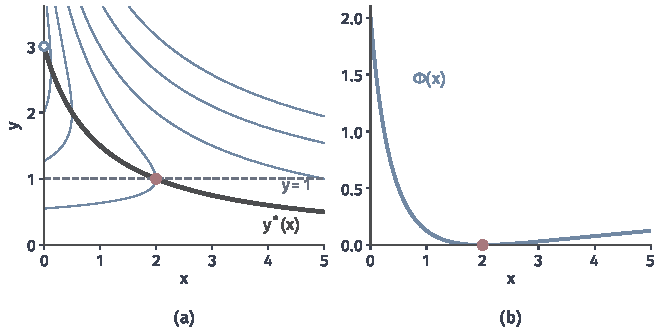
\includegraphics[width=112mm]{figures/05-optimization/07-multiple-criteria-and-nested-optimization/matplotlib/bilevel-reaction/figure.pdf}
 \caption{正则拟合例~\eqref{eq:bilevel-ridge}。(a)蓝色细线是内层目标$g$的等高线，空心点$(0,3)$是$g$对$(x,y)$的最小点；深灰粗线是内解曲线$y^\star(x)=3/(1+x)$；虚线$y=1$上$F$取最小值；红点$(2,1)$是双层问题的解。(b)外层目标$\Phi(x)$，最小点是$x=2$。}
 \label{fig:bilevel-reaction}
\end{BookInlineFigure}

\paragraph{直接作用的例子}
式~\eqref{eq:bilevel-ridge}中$F$不含$x$，全部变化都来自响应。若外层再为$x$付出代价，比如把$F$换成$\frac12(y-1)^2+\frac{1}{10}x$，直接作用就出现了：$\Phi$多了一项$\frac{1}{10}x$，最小点从$x=2$向左移动。两个来源在导数中分别对应一项。

这里的$3$和$1$只是两个固定的数，本章把它们当作给定的优化数据。数据该怎样划分，这样选出的$x$有没有统计上的保证，不是优化问题，可参考\BookChapterRef{chap:finite-sample-error-bounds}{卷八第4章“有限样本的误差上界”}。

\subsection{多解选择}
\label{sec:bilevel-selection}

解集可能含有许多点，它们对内层来说一样好，对外层却可能差别很大。这时$F(\bm{x},\bm{y}^\star(\bm{x}))$这个写法失去了意义，必须补充一条规则。

\paragraph{两种选解规则}
可以用一个比喻来理解。外层是提要求的一方，内层是执行的一方，执行方在几个同样好的方案之间不在乎选哪个。外层可以假定执行方会配合自己，也可以防备它选最不利的。这个比喻只用来记住两种规则，数学上并不要求内层真有什么意愿，规则只是对解集中的点作出约定。

\begin{definition}[乐观模型与悲观模型]
\label{def:bilevel-opt-pes}
对$\bm{x}\in\operatorname{dom}\bm{S}$，定义
\begin{align}
 \Phi_{\mathrm{o}}(\bm{x})&=\inf_{\bm{y}\in\bm{S}(\bm{x})}F(\bm{x},\bm{y}),
 \label{eq:bilevel-optimistic}\\
 \Phi_{\mathrm{p}}(\bm{x})&=\sup_{\bm{y}\in\bm{S}(\bm{x})}F(\bm{x},\bm{y}),
 \label{eq:bilevel-pessimistic}
\end{align}
对$\bm{x}\notin\operatorname{dom}\bm{S}$，两者都规定为$+\infty$。在$\bm{C}$上最小化$\Phi_{\mathrm{o}}$称为\term{乐观模型}（optimistic model），最小化$\Phi_{\mathrm{p}}$称为\term{悲观模型}（pessimistic model）。
\end{definition}

空集上的规定要单独写出。按惯例$\sup\varnothing=-\infty$，若照搬，内层无解的$\bm{x}$在悲观模型中外层值是$-\infty$，反而成了最好的选择，这与第~\ref{sec:bilevel-problem}节开头的约定相反。

两个函数处处满足$\Phi_{\mathrm{o}}\leq\Phi_{\mathrm{p}}$，内解唯一时都等于$\Phi$。乐观模型的$\inf$可以和外层的$\inf$合并，于是
\begin{equation}
 \inf_{\bm{x}\in\bm{C}}\Phi_{\mathrm{o}}(\bm{x})=\inf\{F(\bm{x},\bm{y}):\bm{x}\in\bm{C},\ \bm{y}\in\bm{S}(\bm{x})\}.
 \label{eq:bilevel-optimistic-joint}
\end{equation}
乐观模型因而是一个对$(\bm{x},\bm{y})$的联合最小化，可行集是解集的图像。悲观模型夹着一层$\sup$，不能这样合并。

\paragraph{一个手算例子}
取$\bm{C}$和内层可行集都是$[-1,1]$，目标是
\[
 g(x,y)=xy,\qquad F(x,y)=x^2+y.
\]

内层在$[-1,1]$上最小化关于$y$的线性函数，解由$x$的符号决定：
\[
 S(x)=\begin{cases}
 \{1\}, & x<0,\\
 [-1,1], & x=0,\\
 \{-1\}, & x>0.
 \end{cases}
\]

$x\neq0$时只有一个内解，两种模型相同：$x<0$时外层值是$x^2+1$，$x>0$时外层值是$x^2-1$。分歧只在$x=0$，此时整个区间都是内解，$F(0,y)=y$，于是
\[
 \Phi_{\mathrm{o}}(0)=-1,\qquad\Phi_{\mathrm{p}}(0)=1.
\]

图~\ref{fig:bilevel-selection}画出了这个例子。乐观模型在$x=0$取到最小值$-1$，红点就是它的解。悲观模型的下确界同样是$-1$，因为$x\downarrow0$时$x^2-1\to-1$，但这个值取不到：$x=0$处值跳到$1$，$x>0$时值严格大于$-1$。悲观模型没有最优解。

\begin{BookInlineFigure}
 \centering
 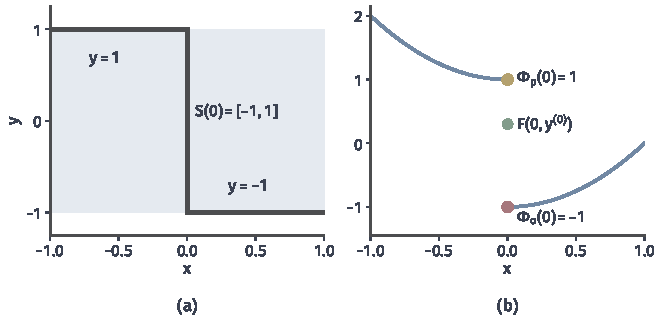
\includegraphics[width=112mm]{figures/05-optimization/07-multiple-criteria-and-nested-optimization/matplotlib/bilevel-selection/figure.pdf}
 \caption{多解时的选解。内层$g=xy$，$x,y\in[-1,1]$，外层$F=x^2+y$。(a)浅蓝是内层可行集，深灰线是解集$S(x)$的图像，$x=0$处是整段区间。(b)蓝线是$x\neq0$时共同的外层值。$x=0$处，红点是乐观值，黄点是悲观值，绿点是从$y^{(0)}=0.3$出发的投影梯度法实际得到的外层值。}
 \label{fig:bilevel-selection}
\end{BookInlineFigure}

\paragraph{乐观模型的解存在，悲观模型没有这样的保证}
上例不是偶然的。把式~\eqref{eq:bilevel-optimistic-joint}看成解集图像上的最小化，就可以套用第~\ref{chap:optimization}章的存在定理，只需说明图像是紧的。

\begin{theorem}[乐观模型解的存在]
\label{thm:bilevel-optimistic-existence}
设$\bm{C}$和$\bm{Y}$是非空紧集，内层可行集恒为$\bm{Y}$，$g$和$F$在$\bm{C}\times\bm{Y}$上连续。则集合
\begin{equation}
 \bm{G}=\{(\bm{x},\bm{y}):\bm{x}\in\bm{C},\ \bm{y}\in\bm{S}(\bm{x})\}
 \label{eq:bilevel-graph}
\end{equation}
非空且紧，乐观模型有最优解。
\end{theorem}

\begin{proof}
对每个$\bm{x}\in\bm{C}$，连续函数$g(\bm{x},\cdot)$在紧集$\bm{Y}$上取得最小值，所以$\bm{S}(\bm{x})$非空，$\bm{G}$非空。$\bm{G}$含于紧集$\bm{C}\times\bm{Y}$，只需证明它是闭集。

取$\bm{G}$中收敛到$(\bm{x},\bm{y})$的序列$(\bm{x}^{(k)},\bm{y}^{(k)})$。$\bm{C}$、$\bm{Y}$闭，所以$\bm{x}\in\bm{C}$，$\bm{y}\in\bm{Y}$。任取比较点$\bm{z}\in\bm{Y}$，由$\bm{y}^{(k)}$是内解，有
\[
 g(\bm{x}^{(k)},\bm{y}^{(k)})\leq g(\bm{x}^{(k)},\bm{z}).
\]

令$k\to\infty$，由$g$连续，得到
\[
 g(\bm{x},\bm{y})\leq g(\bm{x},\bm{z}).
\]
$\bm{z}$是任取的，所以$\bm{y}\in\bm{S}(\bm{x})$，$\bm{G}$是闭集。连续函数$F$在紧集$\bm{G}$上取得最小值，由式~\eqref{eq:bilevel-optimistic-joint}，它就是乐观模型的最优值。
\end{proof}

前面的例子满足定理的全部条件，悲观模型却没有解。原因是第~\ref{chap:optimization}章存在论证的第三关：悲观目标在$x=0$处向上跳，不是下半连续的。

\paragraph{算法的隐含择解}
实际运行时，算法既不会自动做$\inf$，也不会自动做$\sup$。上例中$x=0$时内层梯度是$\partial_yg=x=0$，投影梯度法根本不动，停在初值。从$y^{(0)}=0.3$出发，得到外层值$F(0,0.3)=0.3$，这就是图~\ref{fig:bilevel-selection}(b)的绿点，它既不是乐观值，也不是悲观值。

所以声称求解某个模型时，要说清算法的输出怎样对应这个模型；对应不上的话，算出来的只是“这个算法从这个初值给出的外层值”。

\subsection{有限步内解}
\label{sec:bilevel-finite}

精确内解通常拿不到，实际手里的是算法运行若干步的结果。这个结果也是$\bm{x}$的函数，但它和内解是不同的对象。

\begin{definition}[有限步目标]
\label{def:bilevel-finite}
给定内层算法的初始化和更新规则，把运行$T$步的输出记为$\bm{y}^{(T)}(\bm{x})$。称
\begin{equation}
 \Phi_T(\bm{x})=F(\bm{x},\bm{y}^{(T)}(\bm{x}))
 \label{eq:bilevel-finite-objective}
\end{equation}
为\term{有限步目标}（finite-step objective）。
\end{definition}

这个函数依赖初值、更新规则、步长和步数，换掉任何一项就是另一个函数。

\paragraph{用正则拟合例计算}
对式~\eqref{eq:bilevel-ridge}的内层用梯度下降，初值$y^{(0)}=0$，步长$\alpha=1/2$。内层梯度是$(1+x)y-3$，代入更新式，得到
\[
 y^{(t+1)}=y^{(t)}-\frac12\bigl[(1+x)y^{(t)}-3\bigr]=q\,y^{(t)}+\frac32,\qquad q=\frac{1-x}{2}.
\]

减去不动点$y^\star(x)$，误差每步乘$q$，初始误差是$-y^\star(x)$，所以
\begin{equation}
 y^{(T)}(x)=y^\star(x)\bigl(1-q^T\bigr).
 \label{eq:bilevel-ridge-finite}
\end{equation}

$T$较小时可以写成多项式。前两步的结果是
\[
 y^{(1)}=\frac32,\qquad y^{(2)}=\frac94-\frac34x.
\]

$y^{(1)}$与$x$无关，于是$\Phi_1$是常数，走一步完全看不到$x$的作用。$\Phi_2$的最小点由$y^{(2)}=1$确定，得到$x=5/3$，与$\Phi$的最小点$x=2$不同。

再看$T=3$。直接计算得$y^{(3)}=\frac32(q^2+q+1)$，它在$q=-1/2$时最小，最小值是$9/8$。这时$y^{(3)}$到不了$1$，$\Phi_3$的最小点是$x=2$，最小值却是$1/128$，不是$0$。图~\ref{fig:bilevel-finite-step}比较了几个$T$。

\begin{BookInlineFigure}
 \centering
 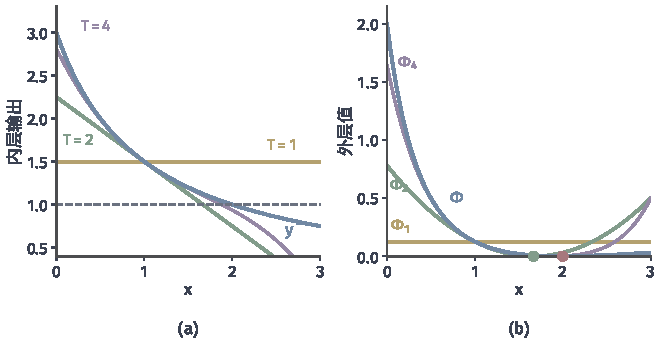
\includegraphics[width=112mm]{figures/05-optimization/07-multiple-criteria-and-nested-optimization/matplotlib/bilevel-finite-step/figure.pdf}
 \caption{有限步内解与有限步目标，内层梯度下降取$y^{(0)}=0$、$\alpha=1/2$。(a)内层输出$y^{(T)}(x)$（$T=1,2,4$）与精确内解$y^\star(x)$（蓝）；所有曲线在$x=1$相交，因为此时$q=0$，一步即得精确解。(b)对应的$\Phi_T$与$\Phi$。绿点是$\Phi_2$的最小点$x=5/3$，红点是$\Phi$的最小点$x=2$。}
 \label{fig:bilevel-finite-step}
\end{BookInlineFigure}

\paragraph{设计目标还是近似手段}
这里要区分两种立场。第一种，最终交付的就是“运行$T$步的这个过程”，$T$和初值是设计的一部分，那么$\Phi_T$本身就是要优化的目标，它的梯度是精确的，不必谈$\bm{y}^\star$。第二种，真正关心的是最优选解，$T$步只是不得已的近似，那么$\Phi_T$与$\Phi$的差别就是要核算的误差。

两种立场下同一个数字含义不同，不能因为运行的是优化算法，就把$\bm{y}^{(T)}(\bm{x})$称作$\bm{y}^\star(\bm{x})$。表~\ref{tab:bilevel-objects}列出本节得到的三个对象。

\begin{BookInlineTable}
 \centering
 \begin{tabular}{lll}
  \toprule
  对象 & 需要说明什么 & 依赖\\
  \midrule
  内解唯一的$\Phi$ & 唯一性 & 问题本身\\
  $\Phi_{\mathrm{o}}$、$\Phi_{\mathrm{p}}$ & 乐观或悲观 & 问题与规则\\
  $\Phi_T$ & 初值、更新、步数 & 算法实现\\
  \bottomrule
 \end{tabular}
 \caption{外层目标的三种对象。内层无解的$\bm{x}$不属于前两行的讨论范围。}
 \label{tab:bilevel-objects}
\end{BookInlineTable}
